\section*{Lucrarea de laborator \#2}
\phantomsection

\section{Scopul lucrarii de laborator}
Realizarea un simplu GUI calculator care suporta urmatoarele functii: +, -, /, *, putere, radical, InversareSemn(+/-), operatii cu numere zecimale.

\section{Mersul lucrarii de laborator}
\tab Pe parcursul lucrarii am creat 2 calculatoare. \textbf{Primul} calculator permite
efectuarea operatiilor ca +, -, /, *, putere, radical, InversareSemn(+/-). Operatiile date se pot efectua in lant (nu este necesar mereu sa apasam pe semnul egal).\\
\tab \textbf{Al doilea} calculator permite calcularea expresiilor matematice mai grele. Aici am divizat functionalitatea in 2 parti (cea grafica si insusi algoritmul de
prelucrarea a expresiei pe care l-am facut in fisiere aparte).\\
\\
\section*{Secvente de cod}
\phantomsection

\textbf{Calculator \#1}\\
\\
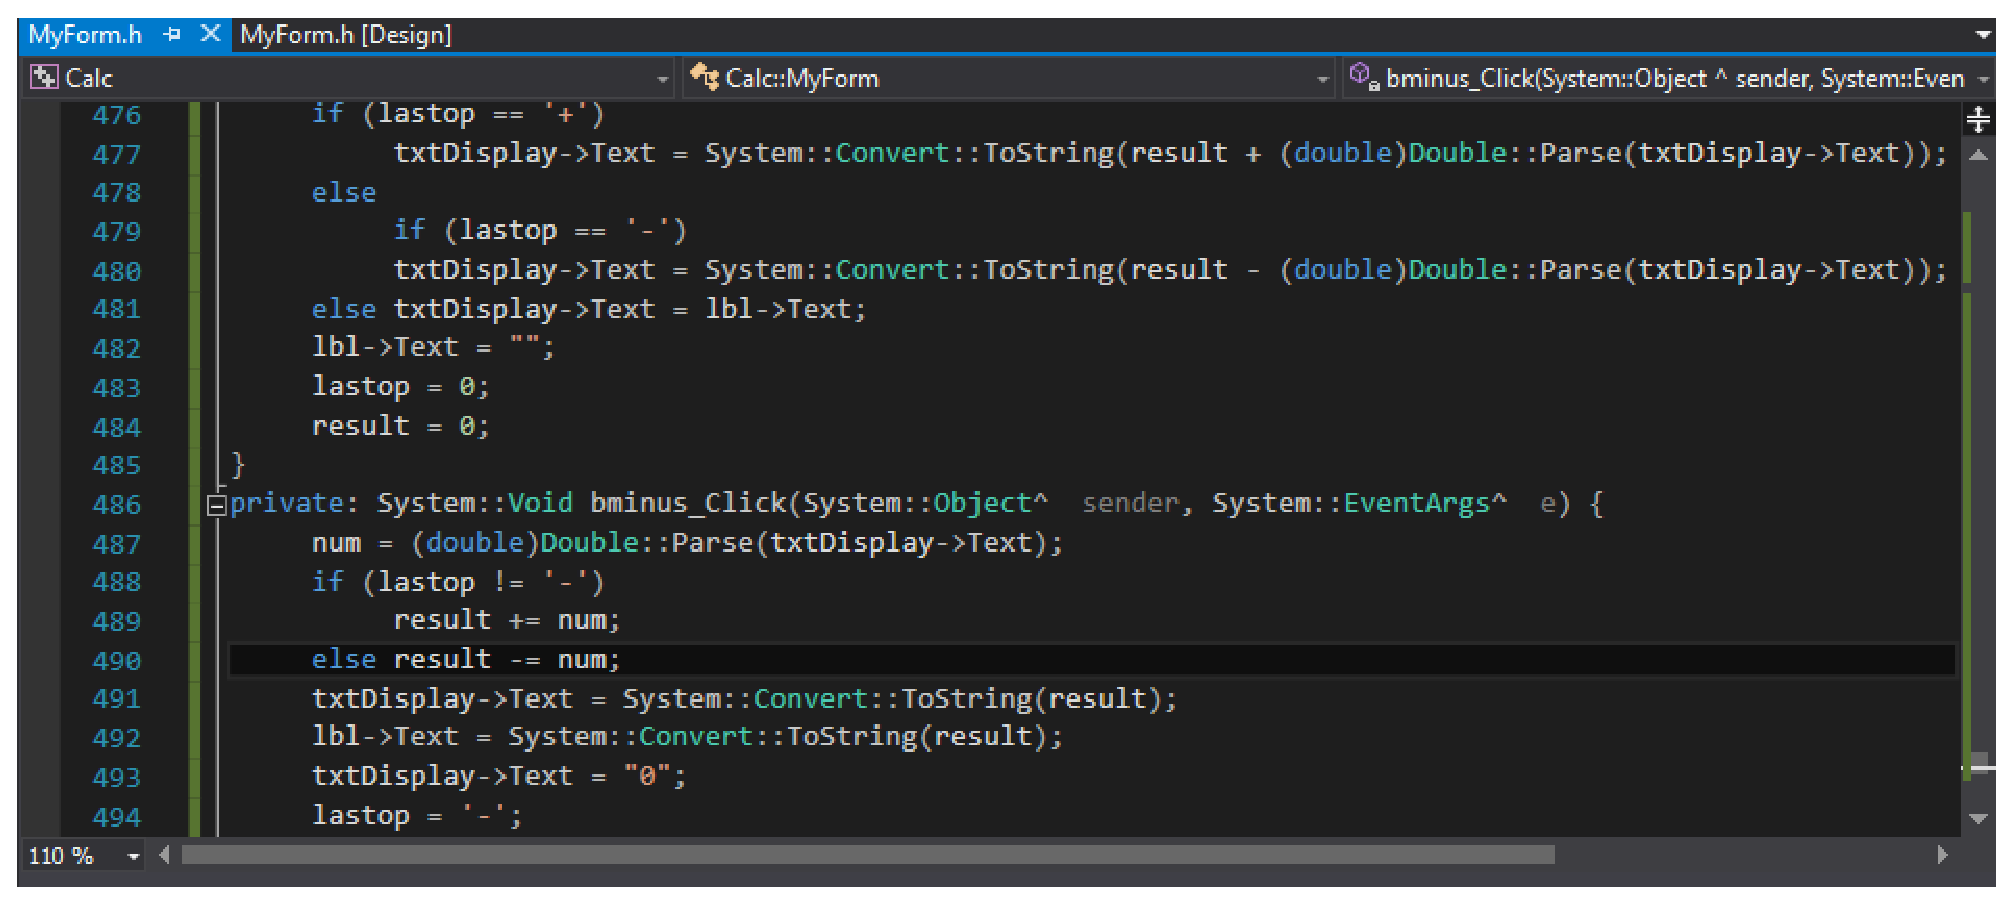
\includegraphics[width=\textwidth]{1.eps}\\
\\
\textbf{Calculator \#2}\\
\\
Partea grafica\\
\\
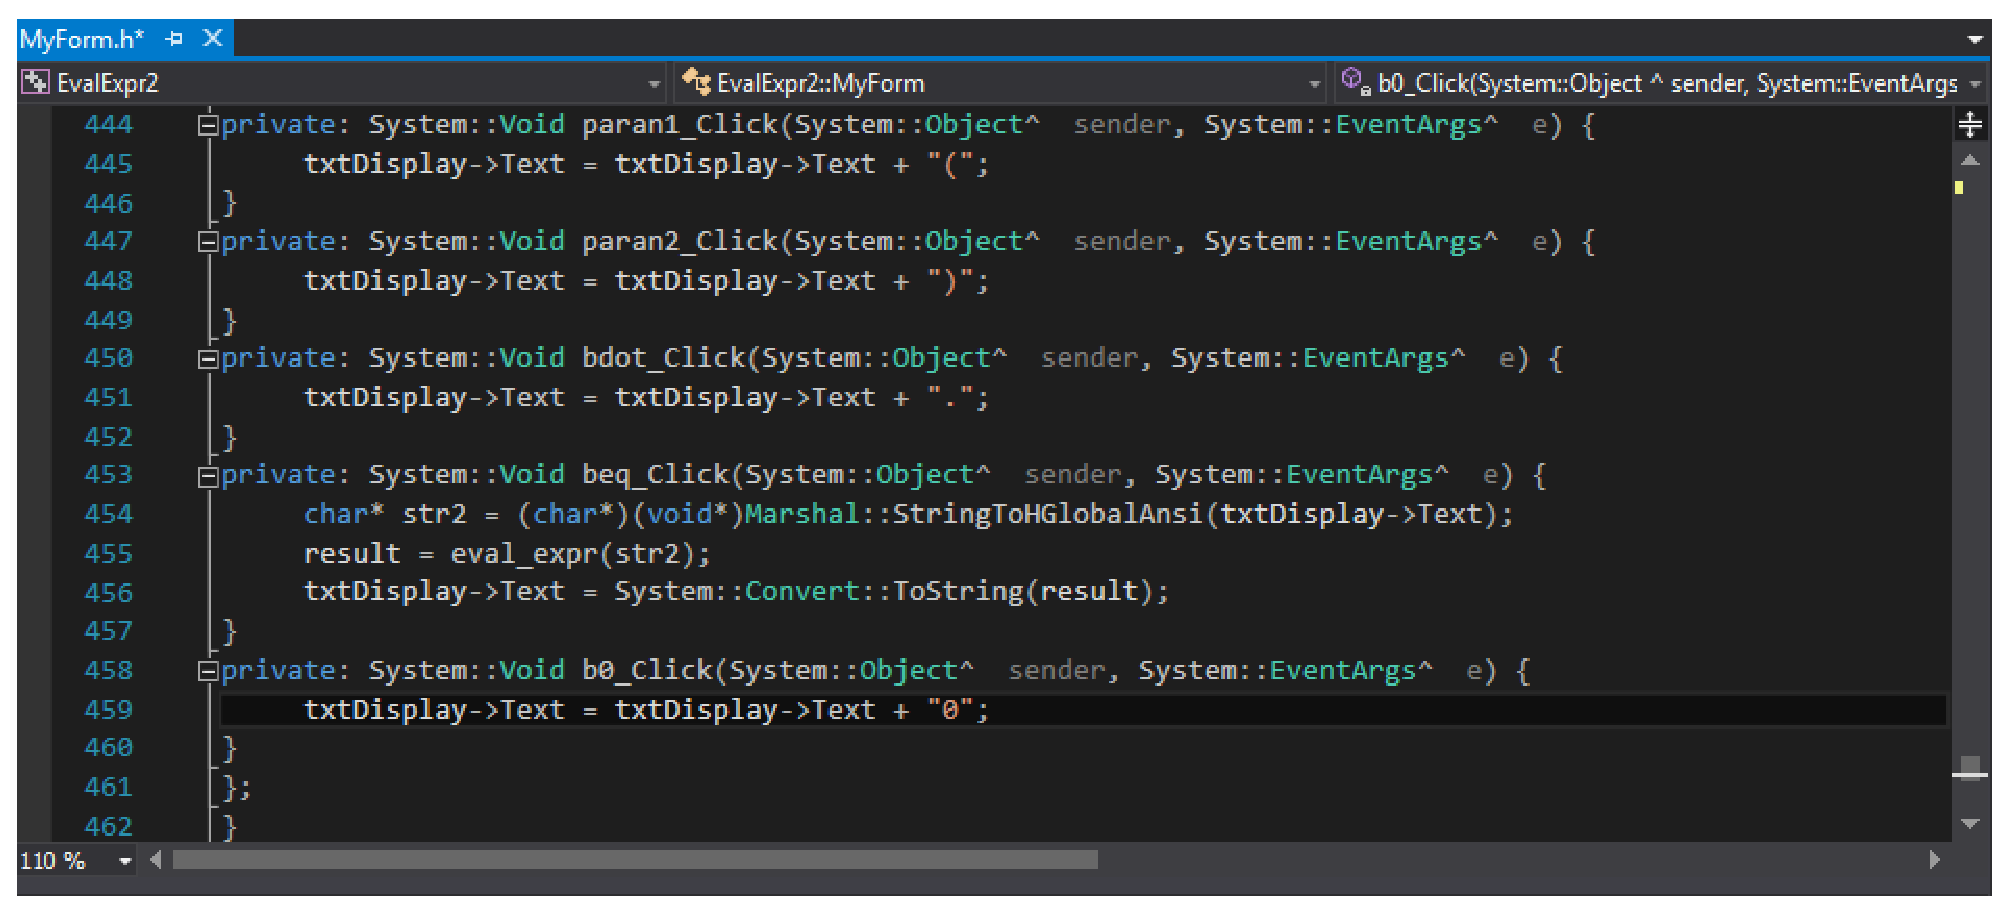
\includegraphics[width=\textwidth]{2.eps}\\
\\
Partea functionala\\
\\
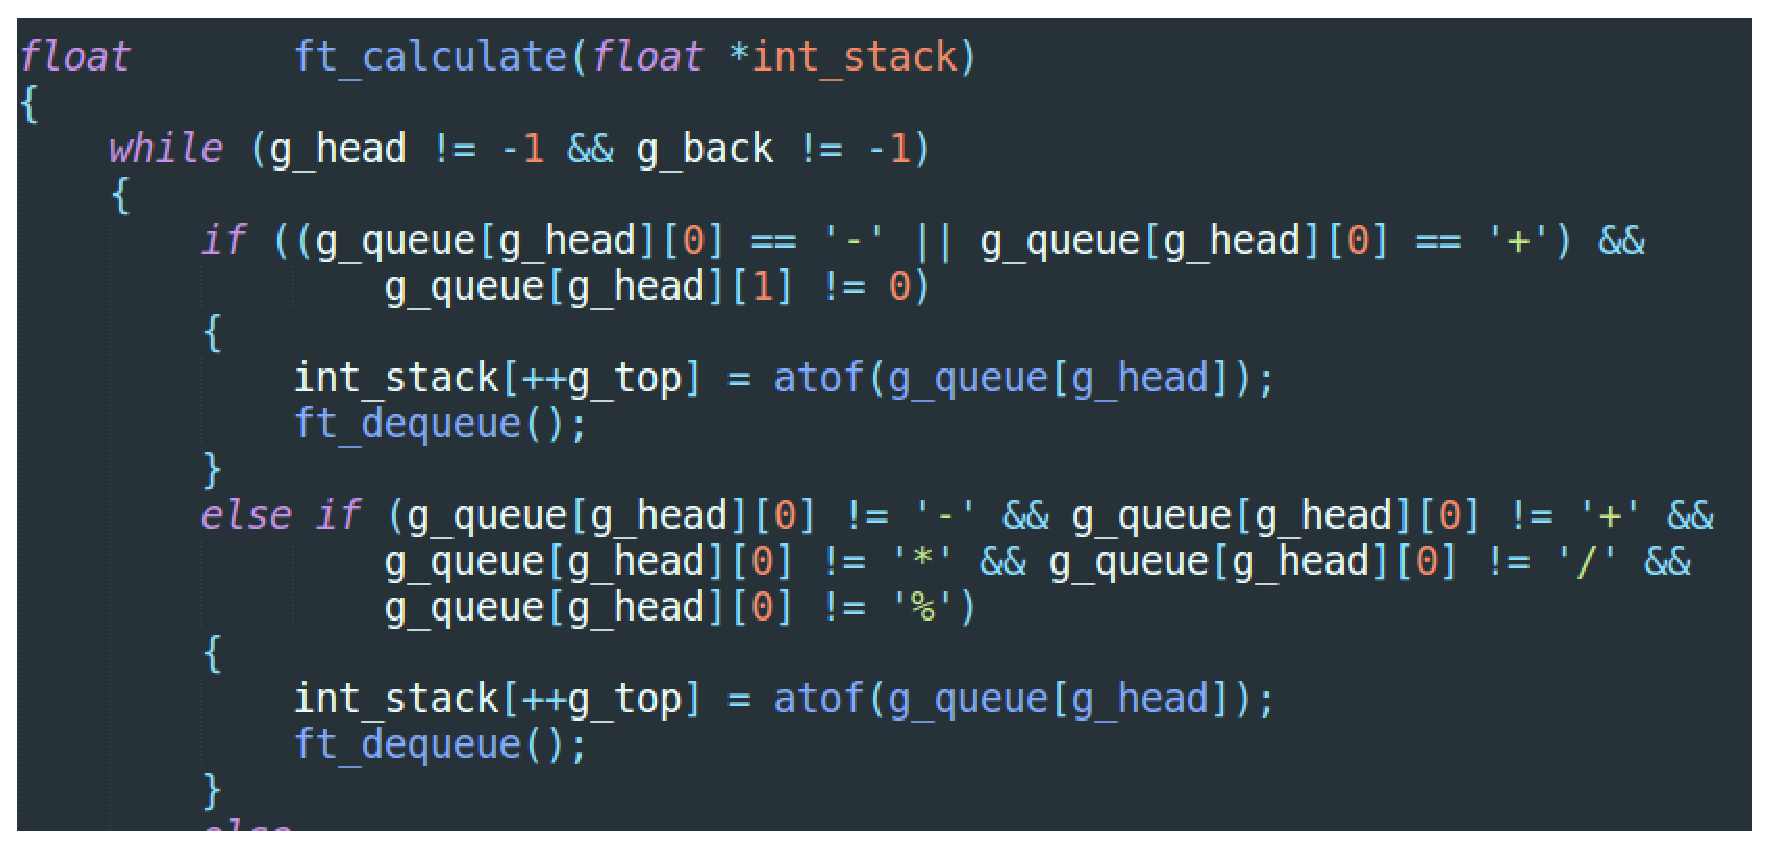
\includegraphics[width=\textwidth]{3.eps}\\
\clearpage
